
\textbf{Reconnaître des solides}\\
On a représenté ci-dessous des solides en perspective cavalière:
\\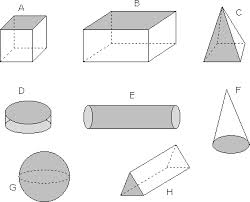
\includegraphics[scale=1.3]{RepS-solides.jpg} 
\\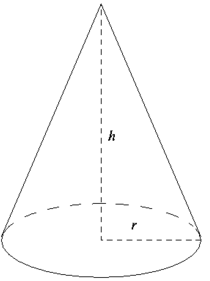
\includegraphics[scale=0.6]{RepS-Cone.png} 
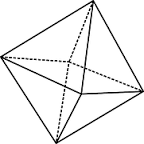
\includegraphics[scale=0.7]{RepS-octaedre.png}
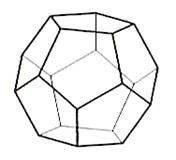
\includegraphics[scale=1]{RepS-ballon.jpg}   

\begin{enumerate}	
	\item Préciser pour chacun son nom, le nombre de faces, le nombres d'arêtes. On pourra compléter le tableau suivant:
\newcolumntype{R}[1]{>{\raggedleft\arraybackslash}b{#1}}
	\newcolumntype{L}[1]{>{\raggedright\arraybackslash}b{#1}}
	\newcolumntype{C}[1]{>{\centering\arraybackslash}b{#1}}
	
	\begin{tabular}{|L{1cm}||C{2cm}|C{2cm}|C{4cm}|}
	\hline Numéro&Nombres d'arêtes&Nombre de faces&Nom\\
	\hline A&...&...&...\\
	\hline B&...&...&...\\
	\hline C&...&...&...\\
	\hline D&...&...&...\\
	\hline E&...&...&...\\
	\hline F&...&...&...\\
	\hline G&...&...&...\\
	\hline H&...&...&...\\
	\hline I&...&...&...\\
	\hline J&...&...&...\\
	\hline K&...&...&...\\
	\hline
	\end{tabular}
	\item Quels sont les éléments caractéristiques des \textbf{prismes}? Donner deux exemples.
	\vspace*{2cm}
	\item Quels sont les éléments caractéristiques des \textbf{cylindres}? Donner deux exemples.
	\vspace*{2cm}
	\item Quels sont les éléments caractéristiques des \textbf{pyramides}? Donner deux exemples.
	\vspace*{2cm}
	\item Quels sont les éléments caractéristiques des \textbf{cônes}? Donner deux exemples.
\end{enumerate}